
%Batteries are important

%Use EM to analyze them

%In particular EELS is good

%Want simulations, use DFT
 
%Want better simulations improve core hole method
\setcitestyle{numbers,open={[},close={]}}

The study of lithium materials has become increasingly relevant in recent years \cite{nitta_li-ion_2015}.  In particular, the field has been driven by the need to develop improved  and more cost effective battery materials \cite{nitta_li-ion_2015}.  %Edit
This is in large part due to the increasing demands for electric vehicles and portable electric devices, both of which continue to demand longer lifetimes and faster charging.

% Original: This drive has come largely in part from increasing demands for electric vehicles and portable electrical devices demanding longer lifetimes and faster charging. 

% Reasoning: "largely in part" doesn't quite make sense. "In large part" is a more commonly used phrase that makes more sense.

Despite the fact all aspects of lithium ion batteries are currently being improved upon, theoretical limits have yet to be reached in multiple properties including capacity, charge density, and charge/discharge rates.  In  addition to performance, safety and the ability to reuse or recycle battery materials are also growing regions of study \cite{gaines_future_2014, doughty_general_2012, balakrishnan_safety_2006}.  % Is this last sentence necessary? You don't seem to ever go back to it, and it's not the most relevant to what you were saying before it. \\ 

As the third element on the periodic table, Lithium's lightweight and high charge density provide great advantages for in the realm of battery performance. In addition to allowing for its batteries to be smaller and lighter without sacrificing lifetime, its small ion size also allows for it to be highly mobile, which in turn leads to superior discharge rates. Furthermore, as an alkali earth metal with a single weakly bound valence electron, lithium is highly electropositive.  As a result, lithium ion batteries can achieve higher operating voltages than its alternatives, such as nickle-cadmium or lead-acid batteries \cite{etacheri_challenges_2011}.  These comparative performance advantages to these alternatives are illustrated in Fig \ref{ragone} \cite{etacheri_challenges_2011}.\\

% Original: In the realm of performance, lithium ion batteries offer a wide range of advantages.  Lithium is the third element on the periodic table and is lightweight  with a very high charge densities.  This allows for batteries to be smaller and lighter without sacrificing lifetime.  Additionally, lithium's lightweight nature and small ion size make it highly mobile, which leads to superior discharge rates. Finally, as an alkali earth metal with a single weakly bound valence electron, lithium is highly electropositive  allowing lithium ion batteries to achieve higher operating voltages than alternatives such as nickle-cadmium or lead-acid batteries \cite{etacheri_challenges_2011}.  These comparative performance advantages to these alternatives are illustrated in Fig \ref{ragone} \cite{etacheri_challenges_2011}.\\

% Reason: In general, it seems your topic sentence of each paragraph is just filler, while your second sentence is your real topic sentence. Once you set what this paragraph will be about, it's easier for the reader to follow.

\begin{figure}
	\centering
	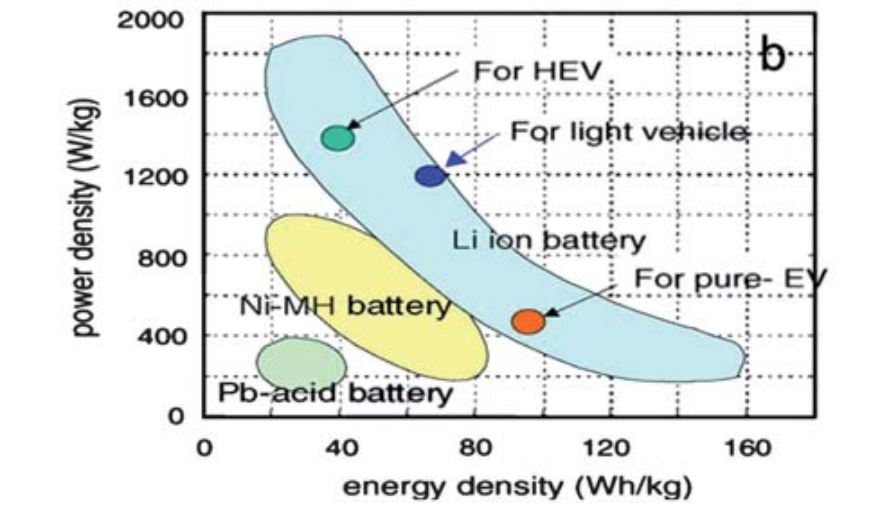
\includegraphics[width=0.5\textwidth]{ragone_plot}
\caption{Power and energy densities achievable by three types of batteries, Li-ion, Ni-MH and Pb-acid. It also illustrates the minimum requirements for some electric vehicles, including Hybrid Electric Vehicles (HEV), Plug in Hybrids (light vehicle).From \cite{etacheri_challenges_2011} }
	\label{ragone}
	
\end{figure}
The pursuit of developing new battery materials has shifted analysis increasingly towards studying the microstructure of materials \cite{lu_lithium_2012,arthur_spontaneous_2016, muller_quantification_2018}. % This sentence isn't clear. Shifted what analysis? Microstructure of what materials?
The ability to identify crystal structure, diffusion mechanics, and composition has become an essential element to understanding and tailoring material properties \cite{van_der_ven_first-principles_2001}.  On this front, electron microscopy has become a central technique to this effort 
% You can use "On this front" or "to this effort", but not both.
 \cite{chiu_aqueous_2013,inkson_2_2016}.  Rapidly improving technology, the possibility of atomic level resolution, coupled with the increasing accessibility have made electron microscopy one of the most prevalent techniques for studying nanoscale features in materials \cite{hansen_atomic-resolution_2001}.  % This sentence needs clarification. It's both vague and refers to ideas you have not mentioned at this point.
 In this respect, lithium is at odds with the method.  % The method? You mean electron microscopy?
 Novel battery materials are increasingly intricate and lithium's light weight and ionizable nature make it particularly sensitive to electron beams, requiring indirect analysis \cite{kobayashi_quantitative_2017}.  These properties make electron energy loss spectroscopy (EELS), a low dosage technique that is well suited for light elements such as lithium, attractive for battery material analysis  \cite{Egerton}. Recent advances extending EELS into low voltage STEM have made EELS appropriate for a range of new materials \cite{SU_9000}. % What new materials? This sentence drops off either include a few examples that show why it's relevant or don't include it.
  However, EELS results are largely qualitative and unstudied systems require a degree of theoretical support.  The theoretical support is all the more essential in dealing with novel technique of low voltage EELS required to study fragile lithium materials. % There are some words missing in this sentence, but I can't tell what you're trying to say.
\\
Theoretical support for EELS can come from a number of methods. The most prevalent of these are based in density functional theory (DFT), a first principles approach that requires only the locations of atoms in a crystal to determine material properties \cite{ks_1965, wien2k,elk,exciting, vasp}.  However, results have been limited to qualitative findings, and lithium's lightweight nature further complicates theoretical approaches \cite{mauchamp_ab_2006, mauchamp_local_2008}. Much of the challenge in simulating EELS for lithium lies in the treatment of the electron hole created in excited atoms.  Lithium's few core electrons mean that excitonic effects from the hole will always be present in the spectra.  Current methods in literature lack the subtlety to treat these effects. 

The goal of this work is to calculate meaningful EELS spectra of lithium materials, specifically in the unprecedented context of EELS at 30 keV. To achieve this goal, the focus is on improving the treatment of core electron holes of lithium in DFT simulations.  % Last sentence, "To achieve this goal, the focus is on improving..." is clunky.

The outline of this thesis is as follows: Chapter \ref{literature_review} presents an overview of EELS, DFT and theoretical EELS calculations.  Chapter \ref{methods} describes the improved method developed in this work and Chapter \ref{results} applies the method to a number of lithium materials.  Chapter \ref{conclusion} concludes the results and addresses future work.


